% Copyright (C) 2005-2015 Airbus - EDF - IMACS - Phimeca
% Permission is granted to copy, distribute and/or modify this document
% under the terms of the GNU Free Documentation License, Version 1.2
% or any later version published by the Free Software Foundation;
% with no Invariant Sections, no Front-Cover Texts, and no Back-Cover
% Texts.  A copy of the license is included in the section entitled "GNU
% Free Documentation License".
\renewcommand{\filename}{docUC_InputNoData_CopulaEstimation.tex}
\renewcommand{\filetitle}{UC : Estimation of a Copula from a sample}

% \HeaderNNIILevel
% \HeaderIILevel
\HeaderIIILevel


\label{copula_estimation}


\index{Copula!Estimation from a sample}
\index{Graph Manipulation!Bounding box}
\index{Graph Manipulation!View}
\index{Graph Manipulation!Show}
\index{Fitting Test!QQ-plot}
\index{Fitting Distribution!Parametric method}



The objective of this Use Case is to :
\begin{itemize}
\item fit a copula to a sample : this estimation may be parametric (when using a specific model of copula) or not (when using the Sklar Copula extracted from a non parametric estimation of the multivariate distribution),
\item validate the estimation with a visual test by superposing the iso-curves of the estimated copula and the sample in the rank space.
\end{itemize}


Details on the Maximum Likelihood  Principle may be found in the Reference Guide (\extref{ReferenceGuide}{see files Reference Guide - Step B -- Maximum Likelihood  Principle}{stepB}).\\

Details on the Parametric Estimators used to evaluate the parameters of the copula may be found in the Reference Guide (\extref{ReferenceGuide}{see files Reference Guide - Step B --  Parametric Estimation}{stepB}).\\



\requirements{
  \begin{description}
  \item[$\bullet$] a 2D numerical sample (data) : {\itshape sample}
  \item[type:]  NumericalSample
  \end{description}
}
             {
               \begin{description}
               \item[$\bullet$] some estimations of the copula : {\itshape estimatedParamCop,estimatedSklarCop }
               \item[type:] a Copula
               \end{description}
             }

             \textspace\\
             Python script for this UseCase :

             \inputscript{script_docUC_InputWithData_CopulaEstimation}

             \textspace\\


             Figure \ref{InitCloud} draws the cloud of the sample in the physical  space and  Figure \ref{RankCloud} draws the sample in the rank space. Figure \ref{Superposition} draws the superposition of the sample in the rank space and the iso-curves of the estimated copula.



             \begin{figure}[H]
               \begin{minipage}{10cm}
                 \begin{center}
                   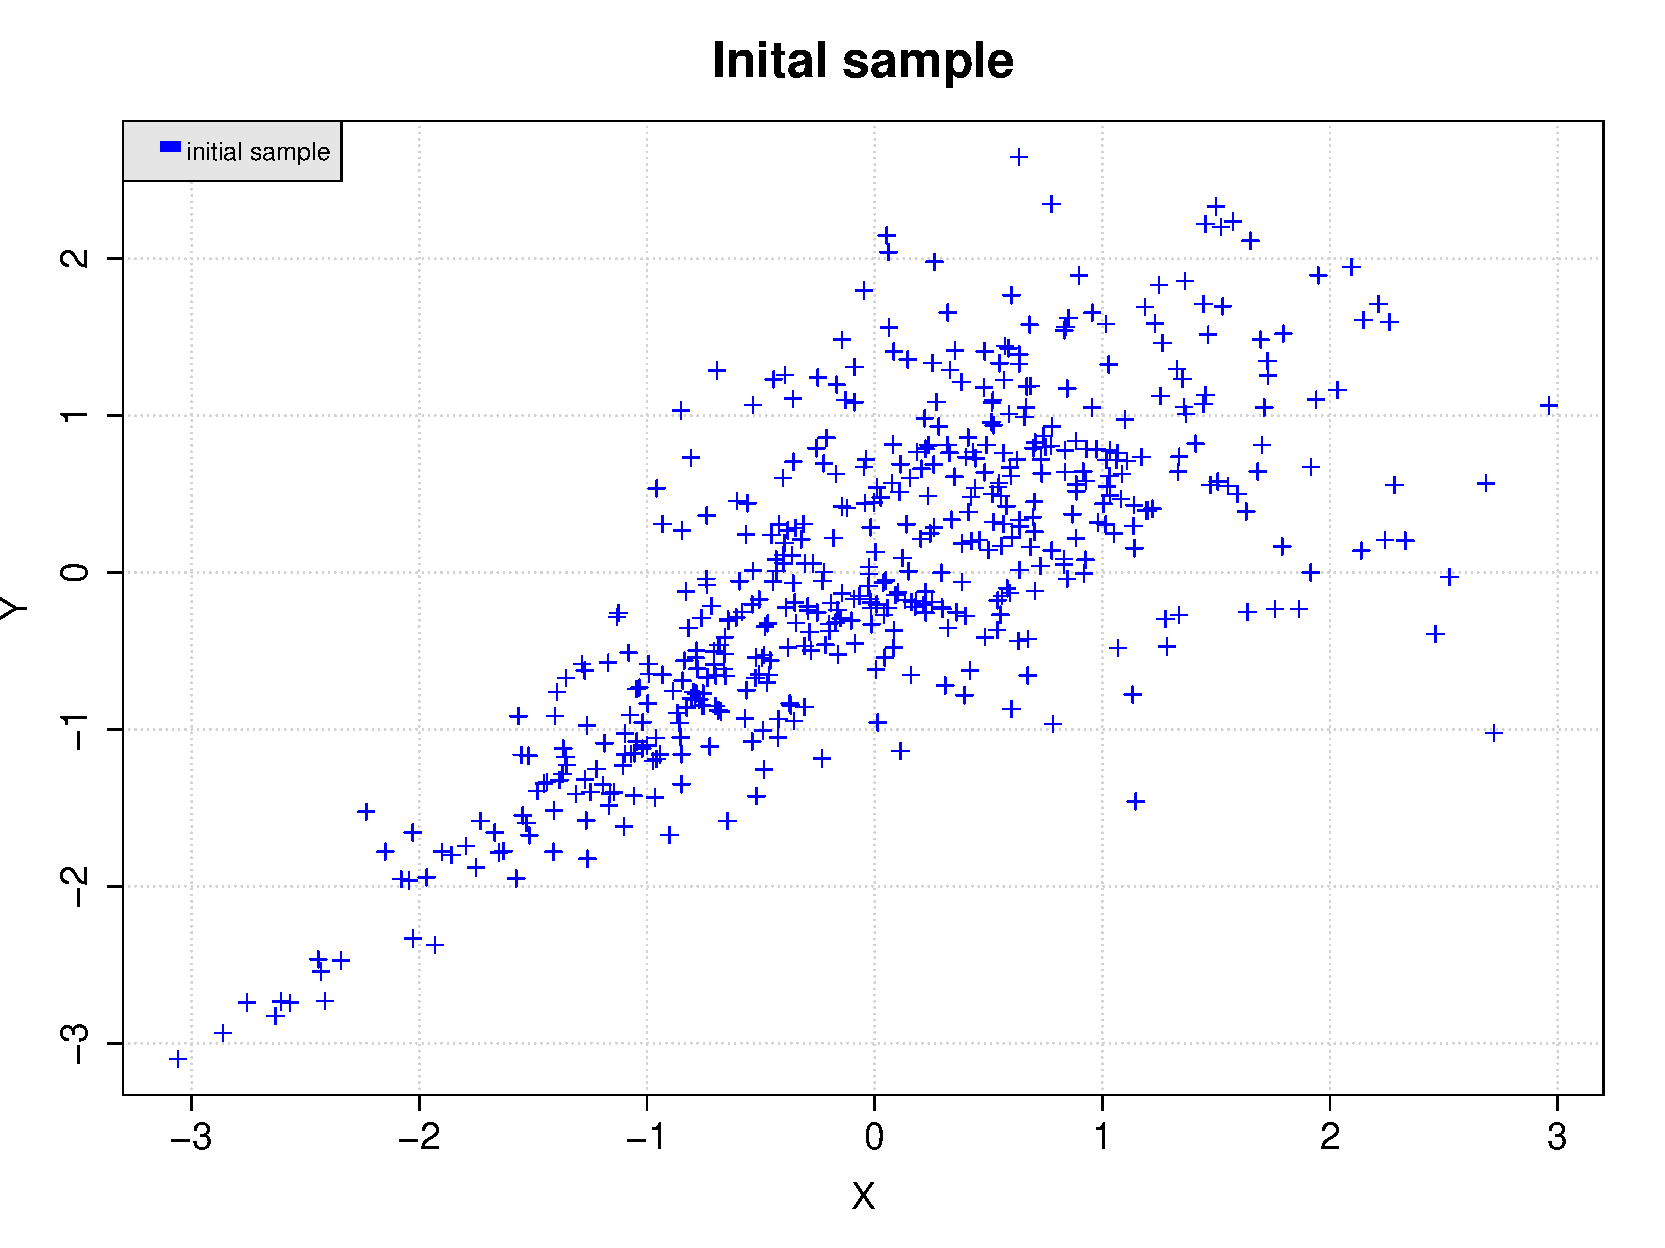
\includegraphics[width=10cm]{Figures/initSample.pdf}
                 \end{center}
                 \caption{Initial sample.}
                 \label{InitCloud}
               \end{minipage}
               \hfill
               \begin{minipage}{10cm}
                 \begin{center}
                   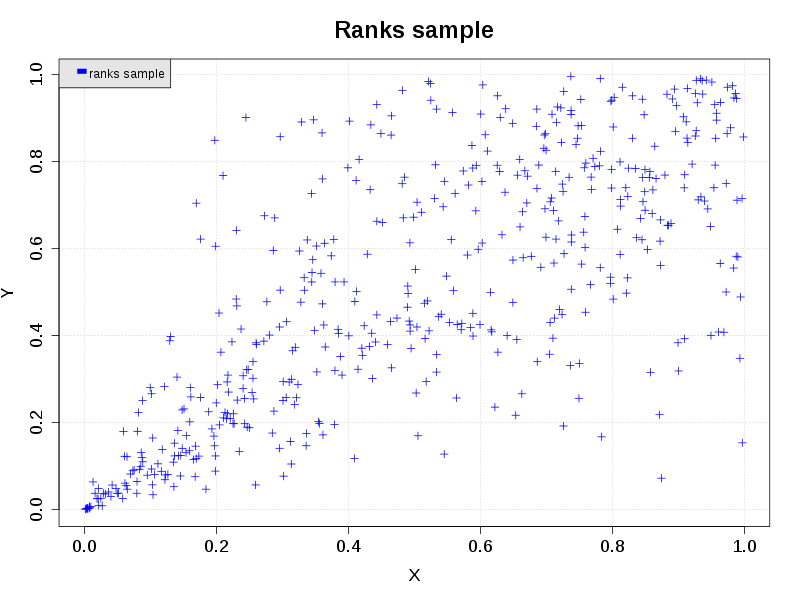
\includegraphics[width=10cm]{Figures/ranksSample.png}
                 \end{center}
                 \caption{Sample in the rank space.}
                 \label{RankCloud}
               \end{minipage}
             \end{figure}


             \begin{figure}[H]
               \begin{center}
                 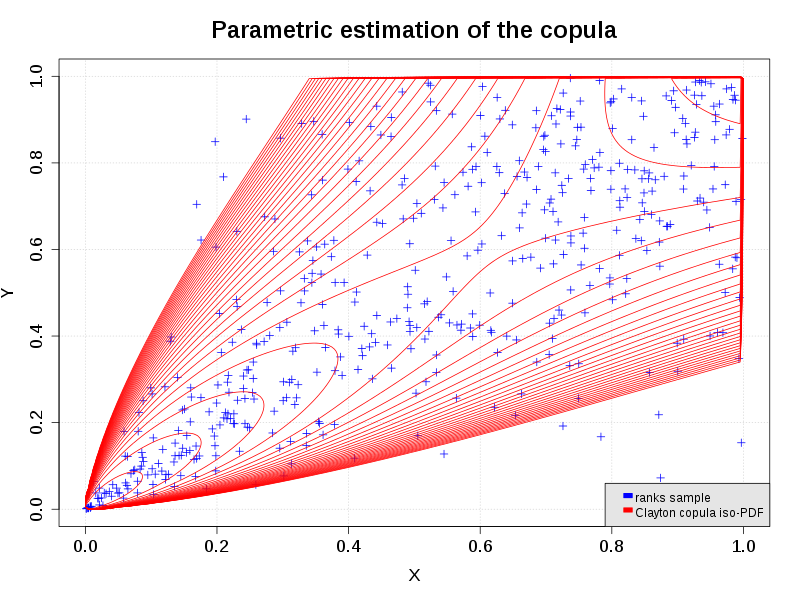
\includegraphics[width=10cm]{Figures/copula_estimation.png}
               \end{center}
               \caption{Sample and iso-PDF curves of the estimated copula.}
               \label{Superposition}
             \end{figure}
